\chapter{Duboko Q učenje (DQN)}
\label{ch:dqn}

Napretkom razvoja neuronskih mreža i rastom njihove popularnosti, nameće se pitanje da li je moguće izvršiti funkcionalnu aproksimaciju funkcije vrednosti stanja ili akcije u stanju koristeći duboke neuronske mreže. Međutim, funkcionalna aproksimacija optimalne funkcije vrednosti akcije u stanju mimo politike nelinearnom funkcijom, kao što je duboka neuronska mreža, nema teorijske ni empirijske garancije, kao što je pokazano u \cite{q_nn_div}.  Termin duboko $q$ učenje (eng.~{\em deep q learning}) odnosi se baš na ovakvo uopštenje algoritma $q$ učenja. Prvi uspešan pristup rešavanju problema učenja potkrepljivanjem na ovaj način prikazan je 2013. godine u radu pod naslovom "Playing atari with deep reinforcement learning" \cite{dqn_mnih}. U radu je predstavljen algoritam kojim, korišćenjem konvolutivne neuronske mreže i još nekih elemenata, agent uspešno uči da igra video igre sa Atari 2600 konzole. Za razliku od nekih ranijih radova, u kojima su bili konstruisani razni atributi na osnovu kojih se uči, u tom radu opisuje se agent koji uči samo na osnovu slike koja je dostupna na ekranu i rezultata u igri, što znači da će se neophodni atributi konstruisati treniranjem neuronske mreže. 
Autori su predstavljeni algoritam imenovali duboko $q$ učenje a neuronsku mrežu koja služi za aproksimaciju duboka $q$ mreža (eng.~{\em Deep $Q$ network}, skr.~{\em DQN}). Baš zbog date mreže koja je deo modela, algoritam se često naziva $DQN$ pa će to biti slučaj i u ovom radu.
\par 
Ovaj rad popraćen je raznim sličnim rezultatima od kojih je verovatno najpoznatiji rad koji je objavio DeepMind, pod naslovom "Human-level control through deep reinforcement learning" ~\cite{dqn_dm}.  U nastavku je opisan algoritam u celosti, kao i unapređenja predstavljena u \cite{dqn_dm}.

\section{Struktura agenta}

Osnovna struktura agenta vodi se idejom $q$ učenja s tim što se za aproksimaciju $q_*$ funkcije koristi neuronska mreža. Uz to, primenjivane su određene tehnika koje osiguravaju stabilnu konvergenciju. 
\par 
Za učenje će biti korišćene četvorke $(s, a, r, s')$ koje predstavljaju deo putanje i koje će biti nazivane prelazima. Glavni elementi sistema za učenje su neuronska mreža koja aproksimira $q$ funkciju i memorija koja čuva već viđene prelaze radi učenja nad njima. U nastavku su opisani ovi elementi i prikaz samog algoritma.

\subsection{Q mreža}
U prethodno razmatranim algoritmima učenja potkrepljivanjem, $q$ funkcija mogla se predstaviti tablicom. Redovi bi označavali stanja a kolone akcije (ili obrnuto) i u njihovom preseku nalazila bi se vrednost akcije u stanju. Dakle, funkcija vrednosti akcije u stanju je funkcija dva argumenta. Umesto tablice, radi treniranja agenta da igra video igru, biće korišćena \textcolor{red}{duboka?} konvolutivna neuronska mreža. Oznaka ove funkcije biće $q_w(s,a)$, gde su $w$ parametri mreže. Prateći terminologiju korišćenu u radovima, mreža će biti nazivana dubokom $q$ mrežom ili samo $q$ mrežom.
\par 
Kao i osnovni algoritam $q$ učenja, $DQN$ će se zasnivati na Belmanovoj jednakosti optimalnosti za $q$ funkciju:
\begin{equation}
	q_*(s,a) = \sum_{s', r}^{} p(s', r~|~s,a)\big[r + \gamma \max_{a'}q_*(s',a')\big]
\end{equation}
Pretpostavlja se da je okruženje determinističko, tj. da ukoliko se u stanju $s$ preduzme akcija $a$, tada se sa verovatnoćom $1$ prelazi u neko drugo stanje $s'$  i dobija nagrada $r$ dok je verovatnoća da se pređe u neko drugo stanje ili da se dobije neka druga nagrada $0$. \textcolor{red}{[OpenAI Gym okruženje dopušta i da ova pretpostavka bude tačna i da bude netačna. Zavisi od frameskip-a. Napisi o ovome negde]}. Prvo pitanje koje treba postaviti jeste kako definisati funkciju greške. Cilj treniranja je približno odrediti optimalnu funkciju vrednosti akcije u stanju, $q_*$. Kako $q_*$ zadovoljava Belmanove jednakosti, teži se tome da njena aproksimacija, $q_w$ približno zadovoljava ove jednakosti. Vodeći se ovom idejom, biće konstruisana funkcija greške, koju treba minimizovati. 
\par 
Za jednu četvorku $s, a, r, s'$ treba minimizovati srednjekvadratnu razliku izraza
\begin{equation}
	q_w(s,a) \text{~i~} \sum_{s', r}^{} p(s', r~|~s,a)\big[r + \gamma \max_{a'}q_w(s',a')\big]
\end{equation}
Međutim, kako funkcija $p$ nije poznata, biće korišćena informacija o tome kolika je nagrada za preduzimanje akcije $a$ u stanju $s$ i koje je novo stanje $s'$. Stoga, drugi izraz postaje
\begin{equation}
	r + \gamma \max_{a'}q_w(s',a')
\end{equation}
gde se pri računanju $q_w(s',a')$ koristi informacija o tome da li je stanje $s'$ završno. Ukoliko jeste, vrednosti $q_w(s',a')$ za sve $a'$ biće $0$. Dakle, funkcija greške može se predstaviti kao očekivanje kvadratne razlike vrednosti $q_w(s,a)$ i $r + \gamma \max_{a'}q_w(s',a')$:
\begin{equation}
	L(w) = \mathbb{E}_{s,a,r,s'}\bigg[ \big(r + \gamma \max_{a'}q_w^-(s',a') - q_w(s,a)\big) ^2 \bigg]
\end{equation} % \frac{1}{2}
Oznaka $q_w^-$ ukazuje na to da se za traženje maksimalne vrednosti akcije u stanju $s$ koriste težine mreže fiksirane pre ažuriranja. Za optimizaciju se koristi stohastički gradijentni spust, opisan u \ref{sss:grad_spust}. Oznaka $\mathbb{E}_{s,a,r,s'}$ označava očekivanje u skladu sa distribucijom iz koje se dobijaju četvorke $(s,a,r,s')$ ali će u praksi ove četvorke biti prikupljane empirijski jer o samoj distribuciji iz koje potiču unapred ne postoje informacije. 
\par 
Još jedan izbor koji treba načiniti vezan je za strukturu izlaza i ulaza u mrežu. Ukoliko se mreža konstruiše tako da kao ulaz prima stanje i preduzetu akciju i kao izlaz daje vrednost dosadašnje aproksimacije, tada bi za odabir najbolje akcije u stanju bilo neophodno propustiti podatke kroz mrežu jednom za svaku akciju. Ovaj pristup mogao bi znatno da uspori obučavanje. S druge strane, moguće je koristiti arhitekturu takvu da mreža kao ulaz primi stanje a kao izlaz da vektor vrednosti za svaku od mogućih akcija. Ova arhitektura biće korišćena u implementaciji.
\par 
U radu koji je objavio DeepMind 2015. godine, predloženo je da se koriste dve mreže, $q$ mreža i ciljna mreža. Težine $q$ mreže biće ažurirane, dok će se izraz $\max_{a'}q_w^-(s',a')$ računati u skladu sa ciljnom mrežom. Na svakih $C$ koraka, težine $q$ mreže kopiraće se u ciljnu mrežu. Ova tehnika osigurava stabilnije učenje i bolje rezultate, kao što je pokazano u \cite{dqn_dm}.

\subsection{Memorija}
Prilikom prikupljanja i korišćenja prelaza za obučavanje treba biti oprezan: ukoliko su uzastopno prikupljene četvorke visoko korelisane, može doći do neefikasnog učenja. Potreba za uklanjanjem visoke korelisanosti uzastopnih prelazaka motiviše korišćenje memorije (eng.~{\em experience replay}~ili~{\em replay memory}) u kojoj će se čuvati ti podaci. Nasumični uzorak iz ove memorije koristiće se za obučavanje Q mreže, čime se smanjuje verovatnoća da je skup podataka nad kojima se vrši ažuriranje parametara korelisan. Memorija ima još jednu ulogu prilikom obučavanja agenta. Naime, uzorkovanjem se prelazi potencijalno više puta koriste za treniranje mreže, što znači da je stopa iskorišćenosti podataka veća. 
\par 
Kako samo treniranje može da bude vrlo dugo, nije izvodljivo čuvati sve prelaze viđene do nekog trenutka već samo poslednjih $N$. Veličina memorije je jedan od metaparametara modela.

\subsection{Dodatni elementi}
\label{ss:dod_el}
\textcolor{red}{Možda deo \ref{ss:dod_el} da se prebaci u detalje implementacije?}
\par 
Za optimizaciju se koristi algoritam RMSProp (\ref{sss:rmsprop}). Nakon računanja, vrši se pojedinačno odsecanje vrednosti gradijenta na interval $[-1, 1]$. Ova tehnika korišćena je u pomenutim radova zbog potencijalnog velikog rasta samog gradijenta koji može da izazove velike eksplozije u vrednostima parametara mreže.
\par 
Kako su ove tehnike ispitivane na mnoštvu igara sa Atari 2600 konzole, nagrade koje su dobijene od okruženja mogu znatno da variraju. Stoga, sve nagrade takođe su odsecane tako da pripadaju $[-1, 1]$. Nažalost, ovo onemogućava razlikovanje većih i manjih nagrada, što može dovesti do manje efikasnog učenja.
\par 
Kao što je rečeno ranije, $DQN$ agent uči na osnovu nagrada i slika sa ekrana igre. Međutim, jedna slika ne daje mnogo informacija. Na primeru igre Breakout, ukoliko je dostupna samo jedna slika ekrana, nemoguće je odrediti u kom se pravcu kreće loptica, ni kojom brzinom. Isto važi i za pločicu koja služi za odbijanje loptice. Međutim, iz nekoliko uzastopnih slika može se odrediti smer i brzina kretanja loptice i pločice. Na slici \ref{fig:ss} prikazane su četiri uzastopne slike sa ekrana.\footnote{Radi ilustracije, nisu prikazane uzastopne slike već je razlika između njih 7 slika. Prikazivanje uzastopnih slika sa ekrana dalo bi kao rezultat 4 skoro identične slike.} Na slike je primenjeno pretprocesiranje, opisano u \ref{ch:implementacija}, u cilju smanjenja računskih zahteva modela. Takođe, kako igre sa Atari 2600 konzole prikazuju $60$ slika u sekundi (eng.~{\em frame per second},~skr.~{\em fps}) i kako nije realno delati tom frekvencijom, vrši se preskakanje slika (eng.~{\em frame skipping}).

\begin{figure}
	\centering
	\resizebox{.24\linewidth}{!}{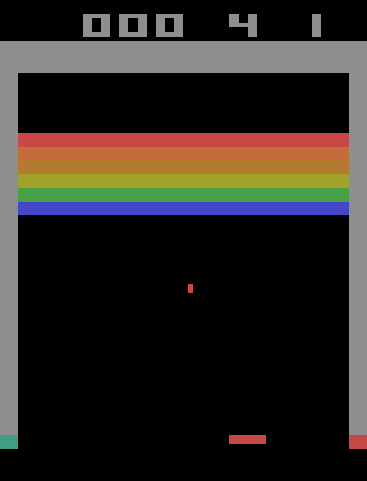
\includegraphics{img/screenshots/1}}
	\resizebox{.24\linewidth}{!}{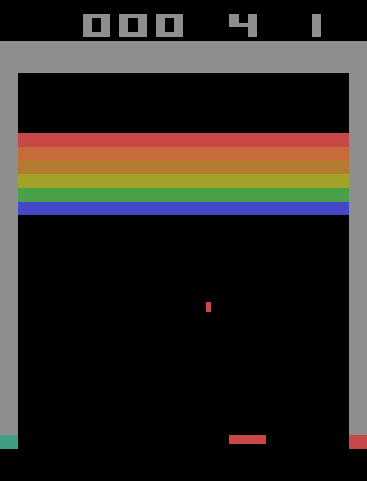
\includegraphics{img/screenshots/2}}
	\resizebox{.24\linewidth}{!}{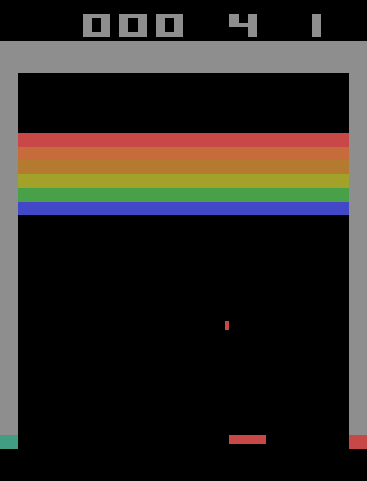
\includegraphics{img/screenshots/3}}
	\resizebox{.24\linewidth}{!}{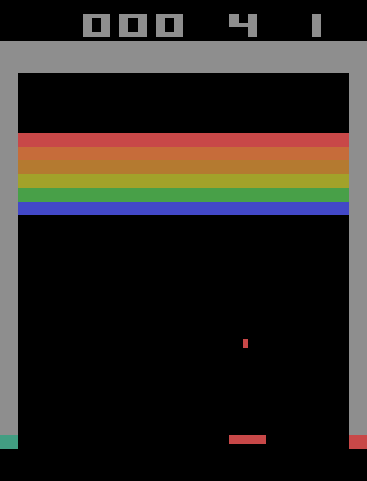
\includegraphics{img/screenshots/4}}
	\caption{Prikaz 4 uzastopna stanja ekrana u igri Breakout. Pločica miruje dok se loptica kreće ka donjem desnom uglu ekrana.}
	\label{fig:ss}
\end{figure}

\section{Algoritam DQN}

Sada su dati svi elementi neophodni za konstrukciju $DQN$ agenta. Algoritam \ref{alg:dqn} okvirno opisuje postupak treniranja DQN agenta. Radi lakšeg razumevanja, dosta detalja je izostavljeno ili izmenjeno. Ti detalji, vezani za konkretnu implementaciju, dati su u \ref{ch:implementacija}. 
\par 
Nomenklatura je sledeća:
\begin{itemize}
	\item $D$ je memorija u kojoj se čuva poslednjih $N$ viđenih prelaza.
	\item $q_w$ je $q$ mreža a $\hat{q}_{\hat{w}}$ je ciljna mreža.
	\item $M$ je broj epizoda koje će se odigrati u toku učenja, a $e$ je broj trenutne epizode. Način na koji se vrši podela na epizode takođe se može naći u detaljima implementacije. 
	\item $t$ je brojač koraka unutar jedne epizode.
	\item $x_t$ je stanje ekrana u koraku $t$.
	\item $s_t$ je stanje u kom se agent nalazi u koraku $t$.
	\item $\phi$ predstavlja funkciju kojom se vrši pretprocesiranje. $\phi_t$ označava pretprocesirano stanje $s_t$.
	\item $C$ je frekvencija ažuriranja parametara ciljne mreže.
\end{itemize}

\begin{myalgorithm}
\caption{DQN}\label{alg:dqn}
\begin{algorithmic}[0]
\Require
Inicijalizovati memoriju $D$ i postaviti njenu maksimalnu dužinu na $N$ \\ 
Inicijalizovati $q_w$ i $\hat{q}_{\hat{w}}$ mreže istim nasumičnim težinama 
\For {$e=1,...,M$}
	\State $s_1 \gets \{x_1\}$
	\State $\phi_1 \gets \phi(s1)$
	\State $t \gets 1$
	\Repeat
		\State Odabrati $a_t \gets
		\begin{cases} \text{nasumično}&\text{, ~sa verovatnoćom~} \varepsilon  \\
                      \argmax_a q_w(\phi(s_t), a) &\text{, ~inače}
        \end{cases}$
		%\State Sa verovatnoćom $\varepsilon$ odabrati nasumičnu akciju $a_t$
		%\State Inače, odabrati akciju $a_t=\argmax_a q_w(\phi(s_t), a)$
		\State Izrši akciju $a_t$, dobijajući nagradu $r_t$ i sliku ekrana $x_{t+1}$
		\State $s_{t+1} \gets s_t, a_t, x_{t+1}$		
		\State $\phi_{t+1} \gets \phi(s_{t+1})$
		\State Smestiti prelaz $(\phi_t, a_t, r_t, \phi_{t+1})$ u memoriju $D$
		\State Dohvatiti nasumičan skup uzoraka $(\phi_j, a_j, r_j, \phi_{j+1})$ iz memorije $D$
		\State Izračunati 
		$y_j \gets \begin{cases} r_j & \text{, ako je } s_{j+1} \text{ završno stanje}  \\
                      r_j + \gamma \max{a'} \hat{q}_{\hat{w}}(\phi_{j+1}, a') & \text{, inače}
        \end{cases}$
        \State Gradijentnim spustom minimizovati vrednosti $(y_j - q_w(\phi_j, a_j))^2$
        \State Svakih $C$ koraka izvršiti dodelu $\hat{w} \gets w$
        \State $t \gets t+1$
	\Until{stanje $t$ je terminirajuće}
\EndFor
\end{algorithmic}
\end{myalgorithm}

U slučaju da se ne koristi ciljna mreža, za računanje vrednosti $y_j$ koriste se vrednosti $q_w^-(\phi_{j+1}, a')$, izračunate korišćenjem $q$ mreže pre ažuriranja parametara. Tada se takođe ne vrši ažuriranje parametara $\hat{w}$ jer oni ne postoje.



